\documentclass[12pt, landscape]{article}
\usepackage[scaled=0.92]{helvet}
\usepackage{calc}
\usepackage{multicol}
\usepackage[a4paper,margin=3mm,landscape]{geometry}
\usepackage{amsmath,amsthm,amsfonts,amssymb}
\usepackage{color,graphicx,overpic}
\usepackage{hyperref}
\usepackage{newtxtext} 
\usepackage{enumitem}
\usepackage[table, dvipsnames]{xcolor}
\usepackage{mathtools}
\setlist{nosep}
\usepackage{tikz}
\usetikzlibrary{shapes.geometric}
\usepackage{makecell}  % for line break withih tabular

% for including images
\graphicspath{ {./images/} }

\pdfinfo{
  /Title (cs3263-midterm.pdf)
  /Creator (TeX)
  /Producer (pdfTeX 1.40.0)
  /Author (Yu Chenbo)
  /Subject (CS3263)
/Keywords (CS3263, nus, cheatsheet, pdf)}

% Turn off header and footer
\pagestyle{empty}

% redefine section commands to use less space
\makeatletter
\renewcommand{\section}{\@startsection{section}{1}{0mm}%
  {-1ex plus -.5ex minus -.2ex}%
  {0.5ex plus .2ex}%x
{\normalfont\large\bfseries}}
\renewcommand{\subsection}{\@startsection{subsection}{2}{0mm}%
  {-1explus -.5ex minus -.2ex}%
  {0.5ex plus .2ex}%
{\normalfont\normalsize\bfseries}}
\renewcommand{\subsubsection}{\@startsection{subsubsection}{3}{0mm}%
  {-1ex plus -.5ex minus -.2ex}%
  {1ex plus .2ex}%
{\normalfont\small\bfseries}}%
\makeatother

\renewcommand{\familydefault}{\sfdefault}
\renewcommand\rmdefault{\sfdefault}
%  makes nested numbering (e.g. 1.1.1, 1.1.2, etc)
\renewcommand{\labelenumii}{\theenumii}
\renewcommand{\theenumii}{\theenumi.\arabic{enumii}.}
\renewcommand\labelitemii{•}
\renewcommand\labelitemiii{•}

\definecolor{mathblue}{cmyk}{1,.72,0,.38}
\everymath\expandafter{\the\everymath \color{mathblue}}

% Don't print section numbers
\setcounter{secnumdepth}{0}

\setlength{\parindent}{0pt}
\setlength{\parskip}{0pt plus 0.5ex}
%% this changes all items (enumerate and itemize)
\setlength{\leftmargini}{0.5cm}
\setlength{\leftmarginii}{0.5cm}
\setlist[itemize,1]{leftmargin=2mm,labelindent=1mm,labelsep=1mm}
\setlist[itemize,2]{leftmargin=2mm,labelindent=1mm,labelsep=1mm}
\setlist[itemize,3]{leftmargin=2mm,labelindent=1mm,labelsep=1mm}

% adding my commands
\input{../Latex/Util/style-helpers.tex}
\input{../Latex/Util/code.tex}
\input{../Latex/Util/math.tex}
\input{../Latex/Util/joins.tex}
% -----------------------------------------------------------------------

\begin{document}
\raggedright
\footnotesize
\begin{multicols*}{3}

    \setlength{\columnseprule}{0.25pt}
    \setlength{\premulticols}{1pt}
    \setlength{\postmulticols}{1pt}
    \setlength{\multicolsep}{1pt}
    \setlength{\columnsep}{2pt}

    \begin{center}
        \fbox{%
          \parbox{0.8\linewidth}{\centering \textcolor{black}{
              {\Large\textbf{CS3236}}
            \\ \normalsize{AY24/25 SEM 1}}
            \\ {\footnotesize \textcolor{gray}{yyccbb}}
          }%
        }
    \end{center}

    \section{CSP}
    \begin{itemize}
        \item AC3 (Arc Consistency)
        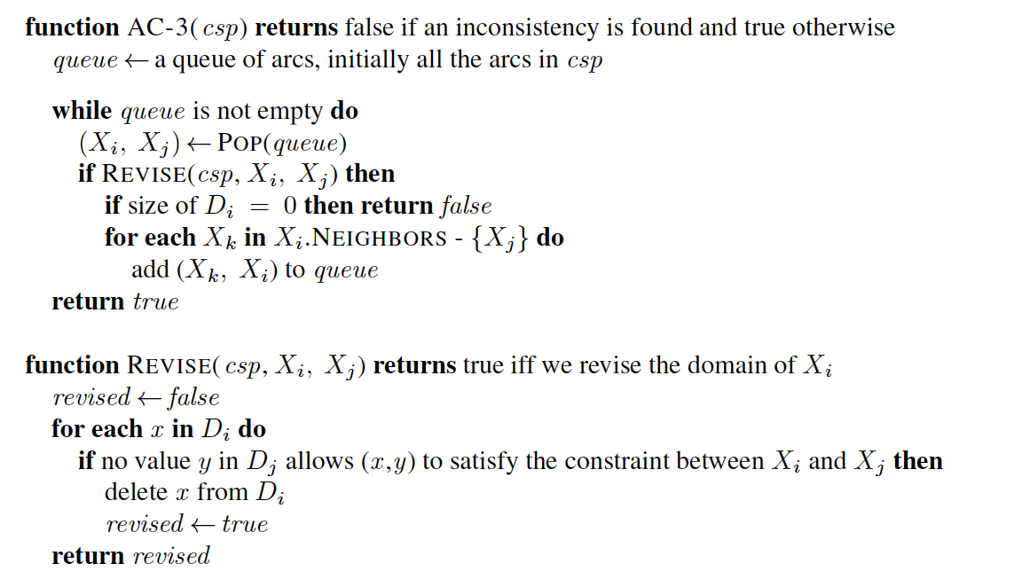
\includegraphics[width=\linewidth]{cs3263-AC3.png}
        \item Backtracking Search
        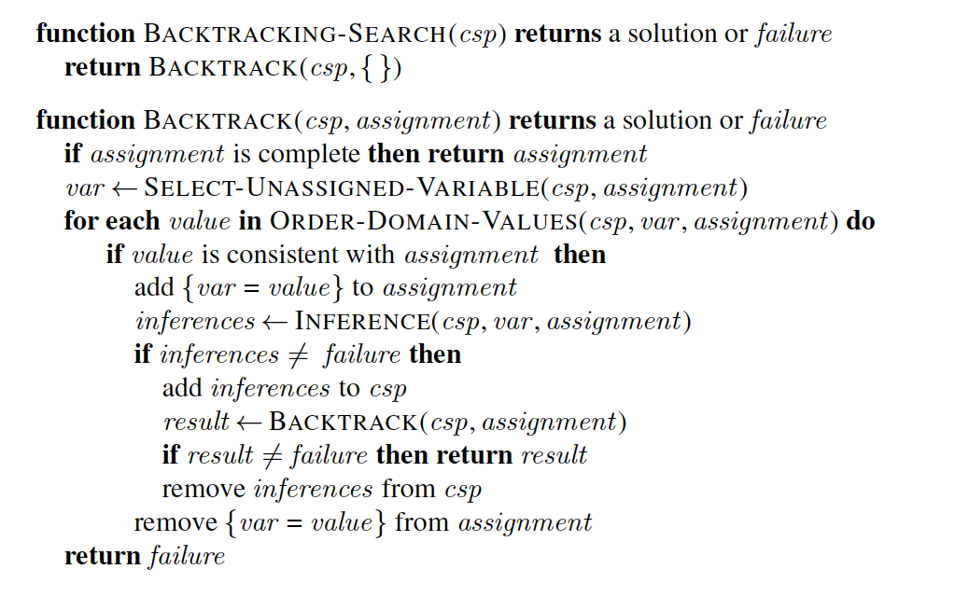
\includegraphics[width=\linewidth]{cs3263-backtracking.png}
        \subsection{Improving Backtracking}
        \begin{itemize}
            \item Variable Ordering (SELECT-UNASSIGNED-VARIABLE): 
            \begin{itemize}
                \item minimum remaining value heuristic 
                \item degree heuristic: choose one with largest number of constraints on other unassigned variables
            \end{itemize}
            \item Value Ordering (ORDER-DOMAIN-VALUES): least constraining value heuristic
            \item Interleaving Seach and Inference:
            \begin{itemize}
                \item Forward Checking: only enforce arc consistency among immediate neighbours
                \item MAC: resursively propagates constraints
            \end{itemize}
            \item Conflict Set Backjumping:
            \begin{itemize}
                \item Conflict set of X: set of assignments which shrink the domain of X
                \item Backjumping: backtrack to the most recent assignment in the conflict set
            \end{itemize}
        \end{itemize}
        % \columnbreak
        \item Min-Conflict Local Search
        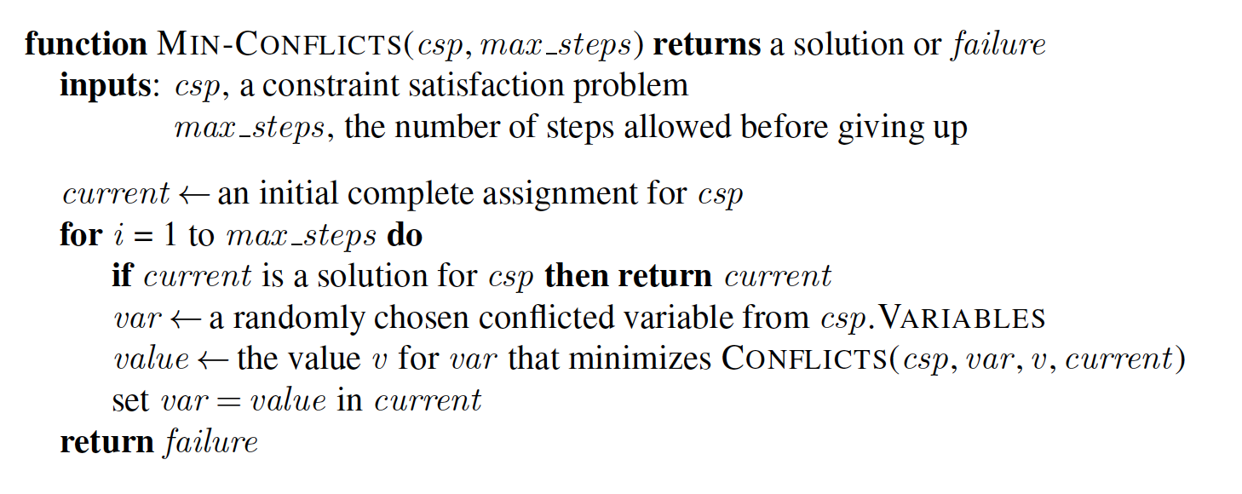
\includegraphics[width=\linewidth]{cs3263-local-search.png}
        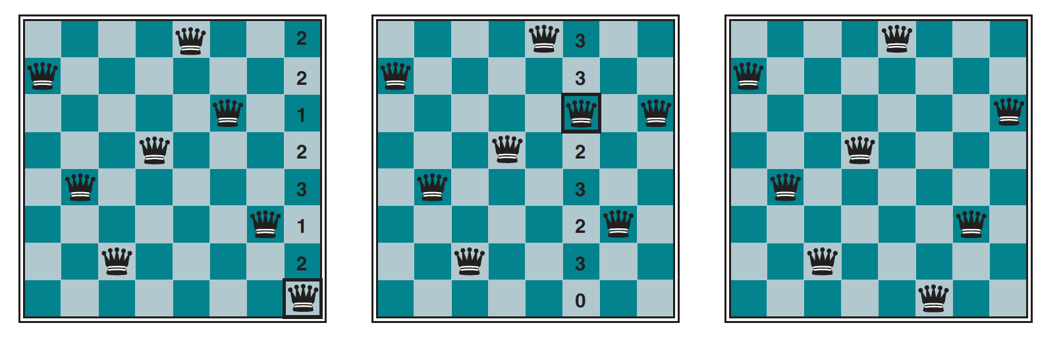
\includegraphics[width=\linewidth]{cs3263-local-search-n-queens.png}
    \end{itemize}

    \section{Propositional Logic}
    \begin{itemize}
        \item \definition[]{Satisfiability} If $\alpha$ is true in m, m satisfies $\alpha$ and m is a model of $\alpha$. $M(\alpha)$ denotes the set of all models of $\alpha$.
        \item \definition[]{Entailment} $\alpha\models\beta$ iff in every model in which $\alpha$ is true, $\beta$ is also true. $M(\alpha)\subseteq M(\beta)$
        \item 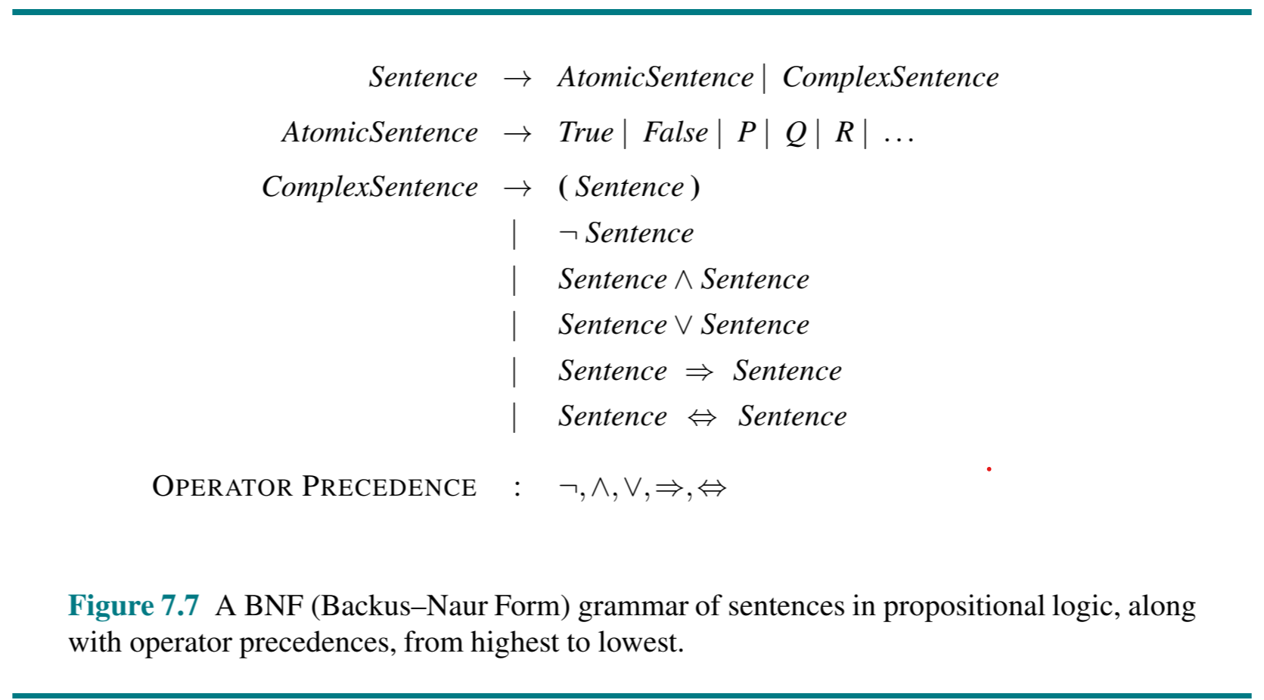
\includegraphics[width=\linewidth]{cs3263-proplogic-syntax.png}
        \item \textbf{Model Checking:} Check for all models of KB (when KB is True)
        \item \textbf{Theorem Proving:}
        \begin{itemize}
            \item $\alpha\models\beta$ iff $\alpha\implies\beta$ iff $\alpha\land\lnot\beta$ is unsat
            \item 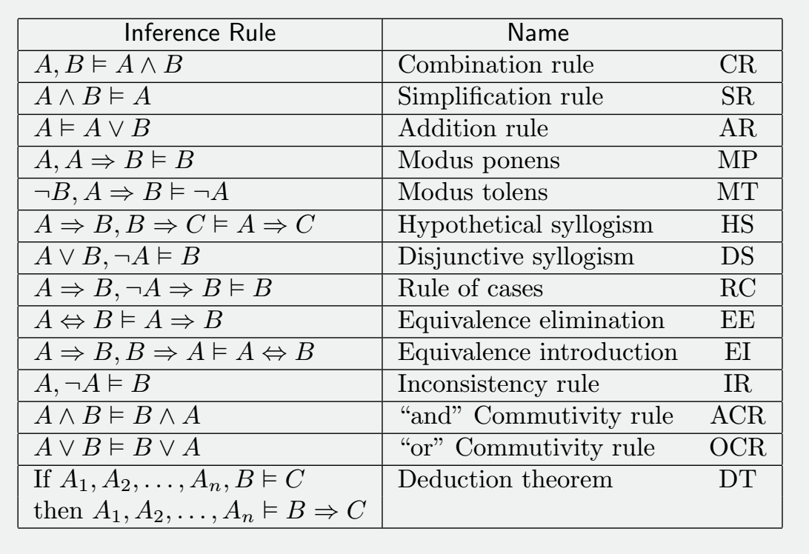
\includegraphics[width=\linewidth]{cs3263-proplogic-deduction-system.png}
        \end{itemize}
        \item \textbf{Resolution:}
        \begin{itemize}
            \item Only applies to CNF
            \item $(A\lor P), (B\lor\lnot P) \models A \lor B$
            \item If A and B have copies of the same literal, remove one.
            \item Algorithm:
            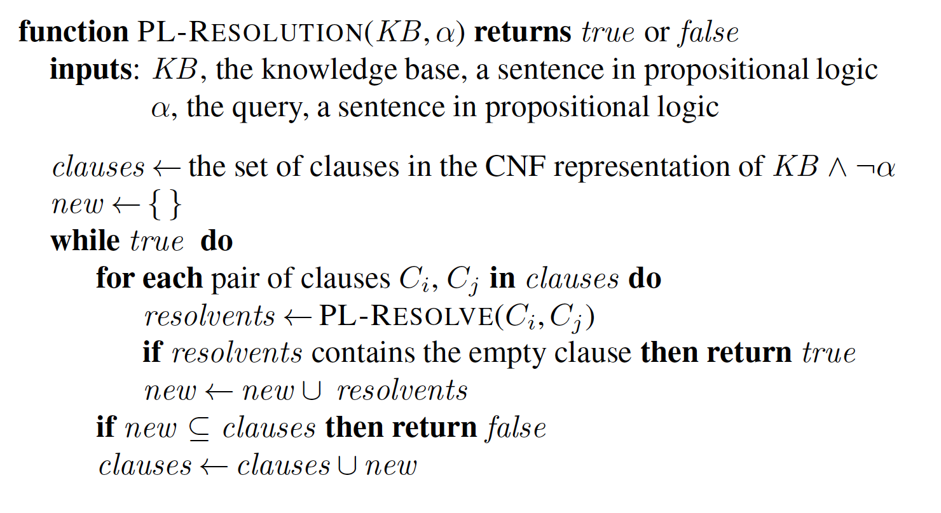
\includegraphics[width=\linewidth]{cs3263-proplogic-resolution.png}
        \end{itemize}
        \item \definition[]{Definite Clause} disjunction of literals where exactly one is positive.
        \item \definition[]{Horn Clause} disjunction of literals where at most one is positive.
        \\ Deciding entailment with pure horn clause KB is linear-time.

    \end{itemize}

    \section{First Order Logic}
    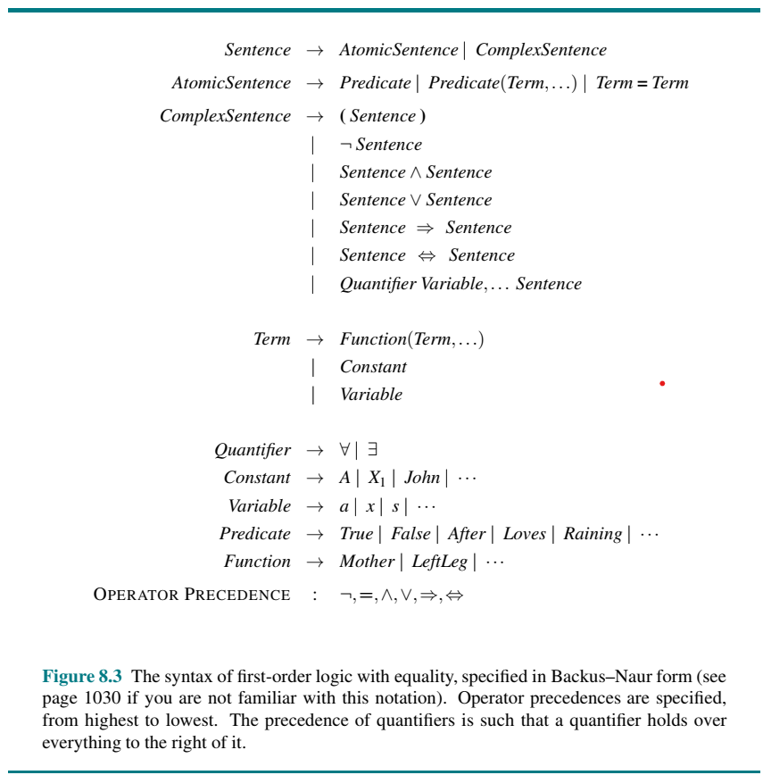
\includegraphics[width=\linewidth]{cs3263-fol-syntax.png}
    \begin{itemize}
        \item \textbf{Universal Instantiation:} $\frac{\forall v \hspace{0.5ex}\alpha}{SUBST({v/g},\alpha)}$
        \item \textbf{Existential Instantiation:} same as UI with g replaced by k, a Skolem constant that does not appear elsewhere in the KB
        \item Caveat for reusing the symbol: UI before EI then it is logically wrong.
        \item \textbf{Unification:}
        \begin{itemize}
            \item a variable cannot be replaced by a term containing itself (e.g. a function of itself)
            \item Most General Unifier (MGU)
            \item 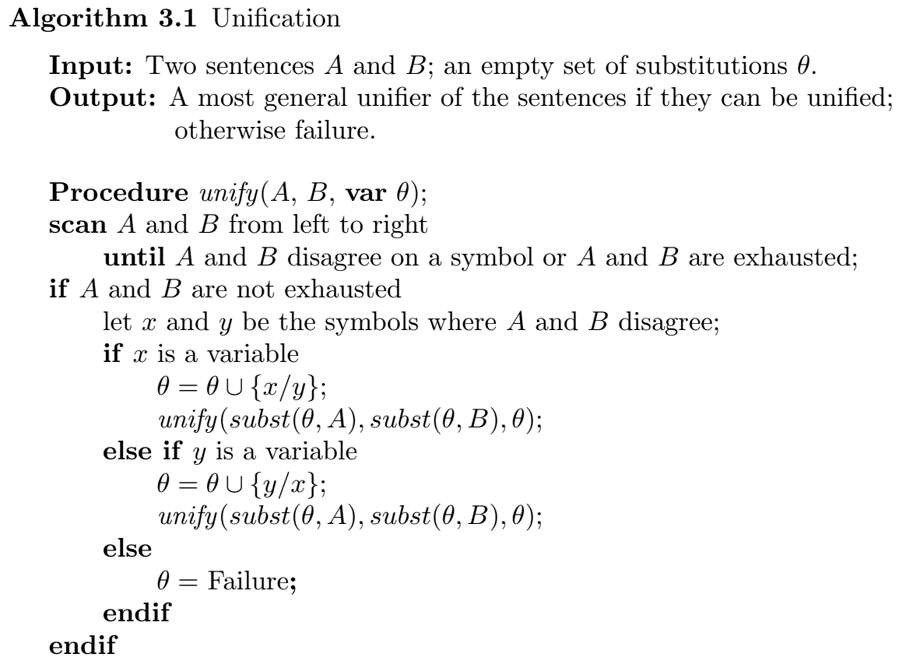
\includegraphics[width=\linewidth]{cs3263-fol-unification.png}
            \item *occur-check needed before each update of $\theta$
            \item 
        \end{itemize}
        \item \textbf{Forward Chaining:}
        \item 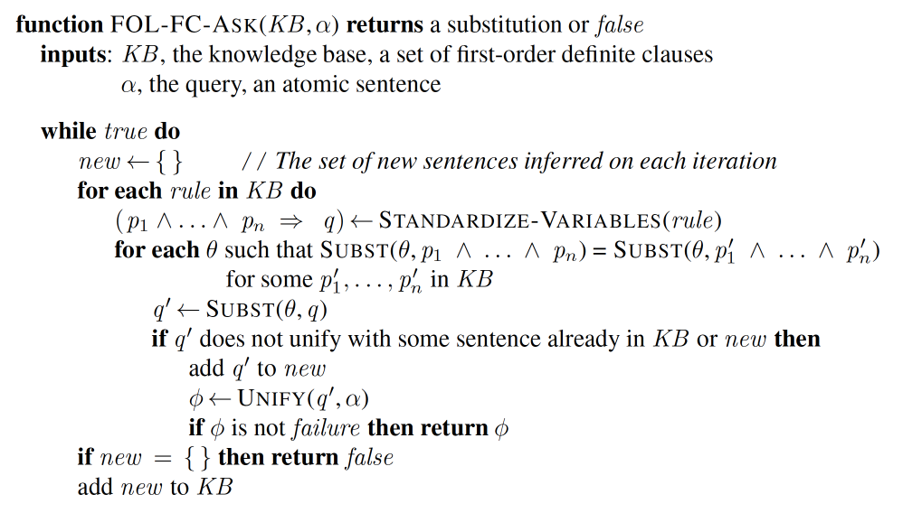
\includegraphics[width=\linewidth]{cs3263-fol-forward.png}
        \item \textbf{Backward Chaining:}
        \item 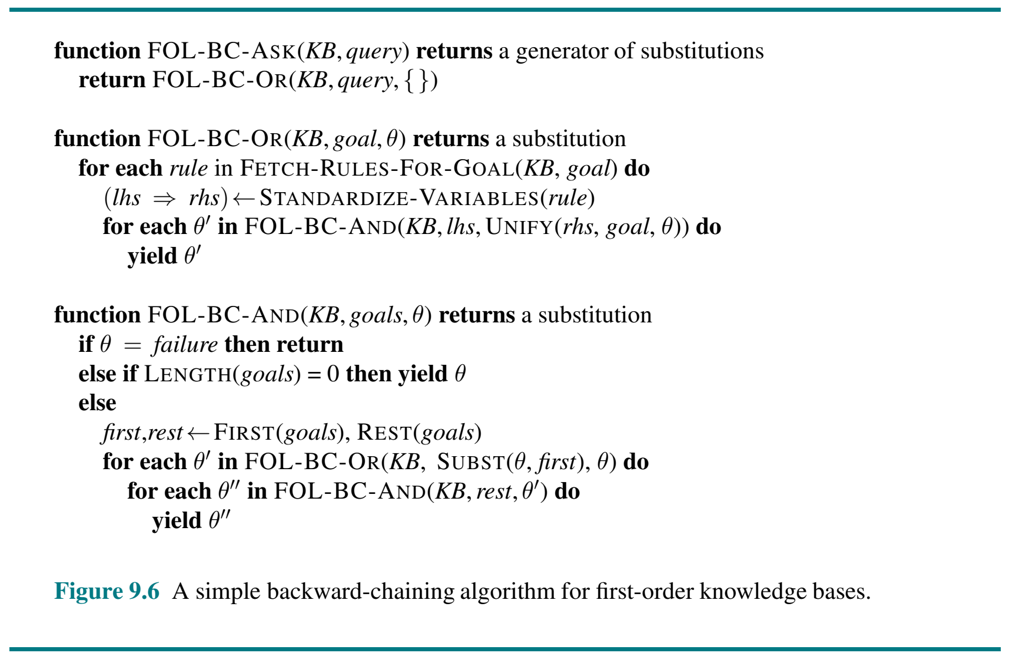
\includegraphics[width=\linewidth]{cs3263-fol-backward.png}
        \item \textbf{Resolution:}
        \item Convert to CNF:
        \begin{itemize}
            \item Use implication rule
            \item Move $\lnot$ inside
            \item Standardise variables: replace repeated variables
            \item Skolemise: translate $\forall x \exists y P(y)$ into $P(F(x))$
            \item Drop universal quantifiers
            \item Distribute disjunction over conjunction
        \end{itemize}
        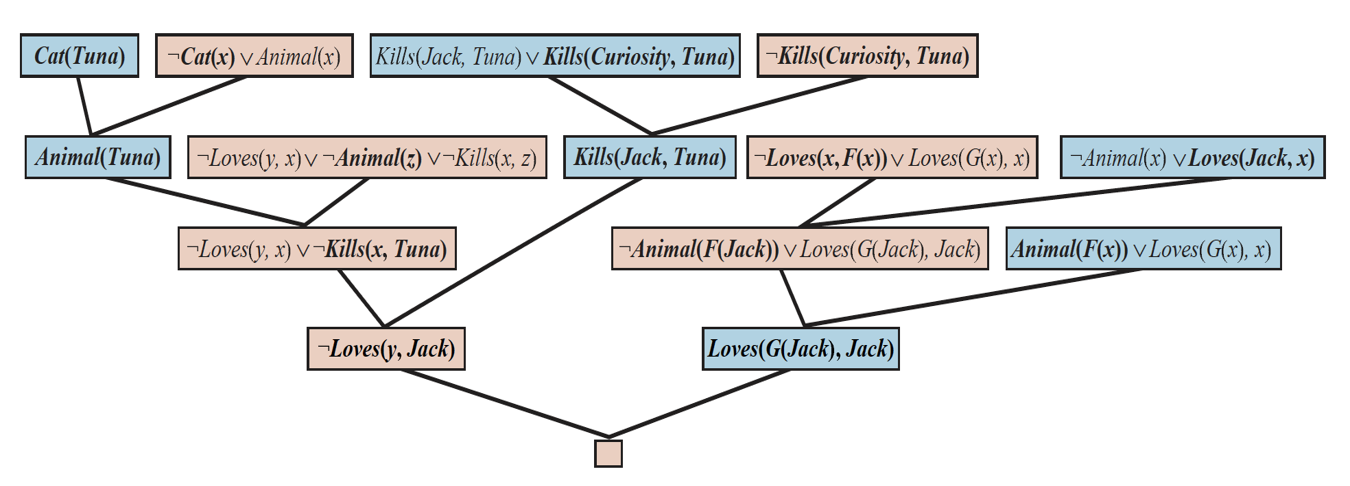
\includegraphics[width=\linewidth]{cs3263-fol-resolution-cat-example.png}
    \end{itemize}

    \section{BN}
    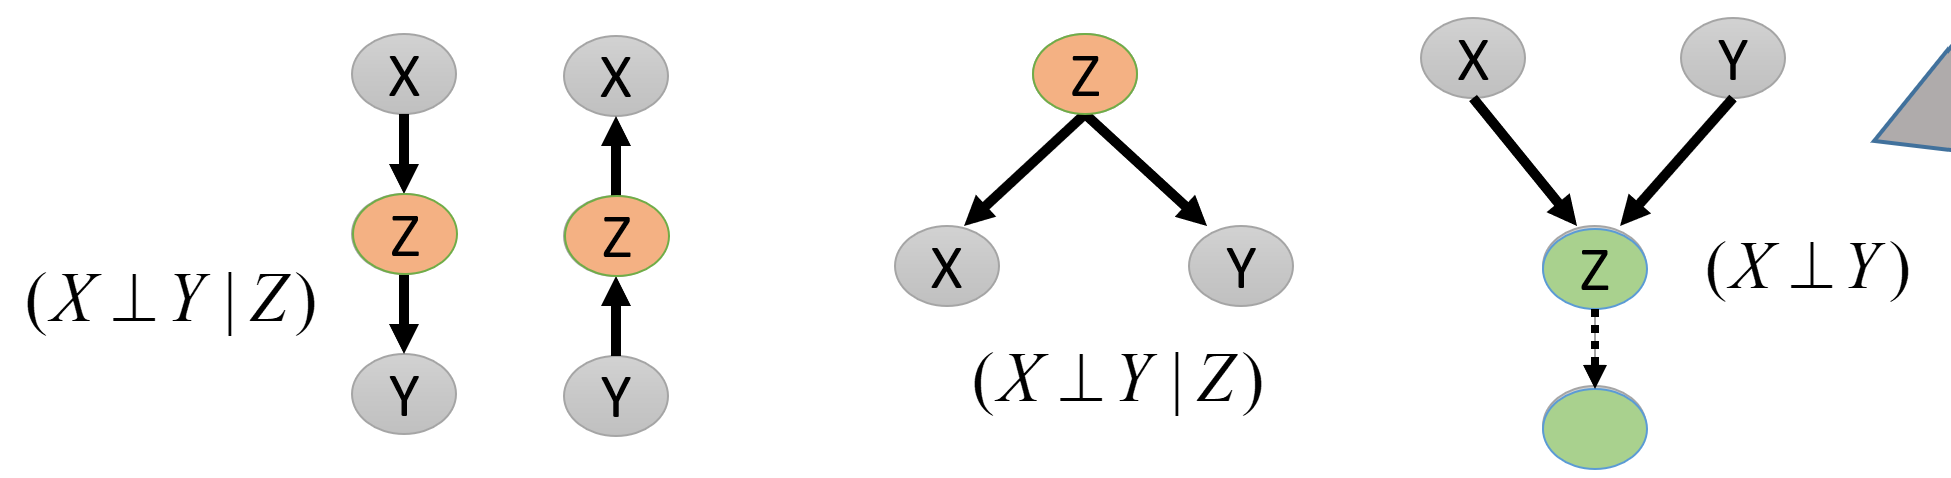
\includegraphics[width=\linewidth]{cs3263-bn-trails.png}
    
\includegraphics[width=0.3\linewidth]{cs3263-bn-trail1.png}
    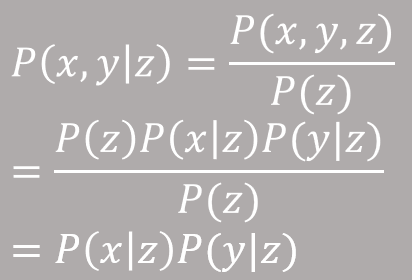
\includegraphics[width=0.3\linewidth]{cs3263-bn-trail2.png}
    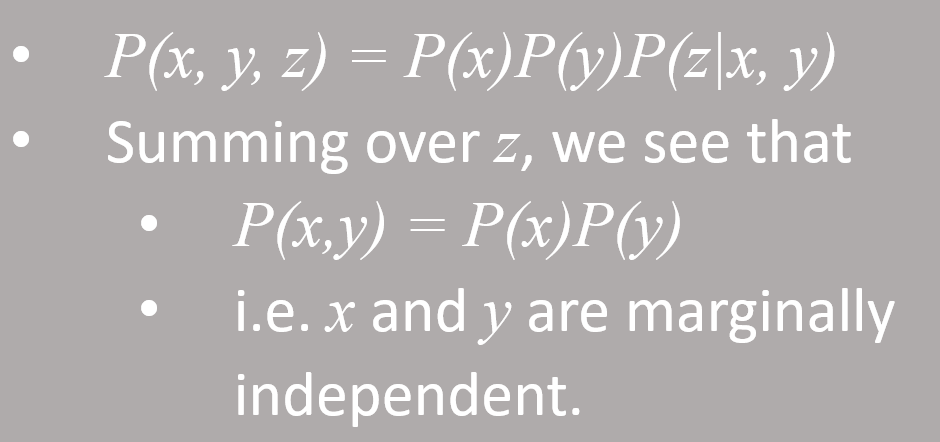
\includegraphics[width=0.3\linewidth]{cs3263-bn-trail3.png}
    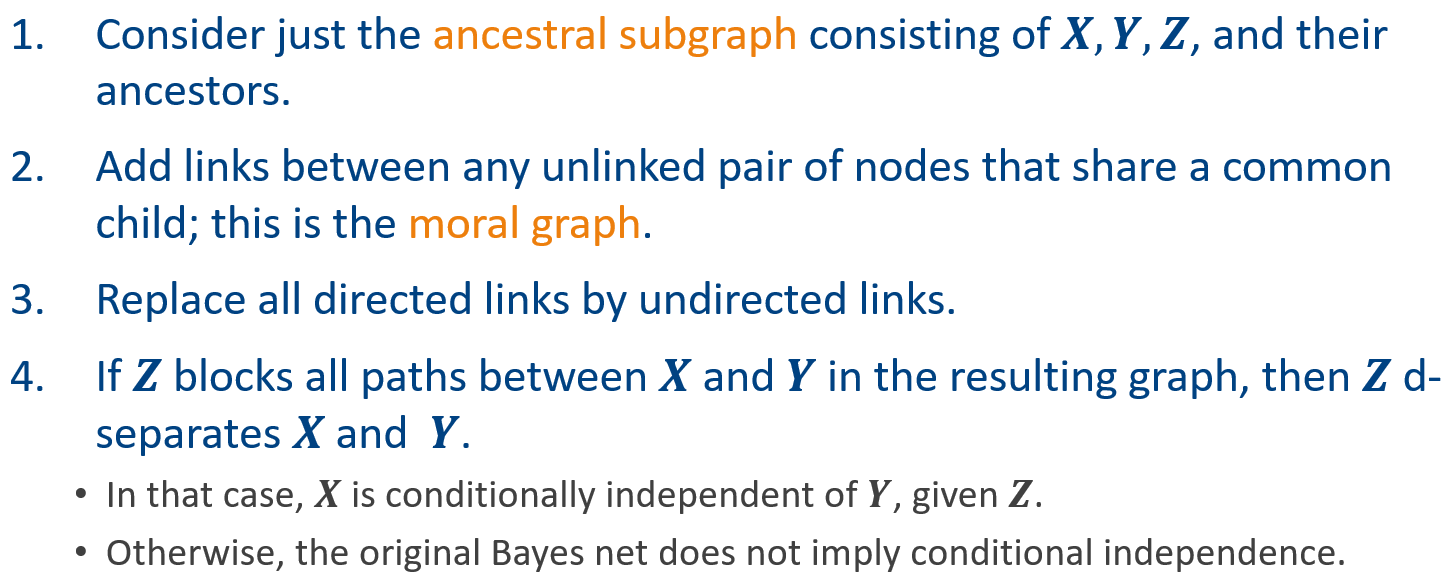
\includegraphics[width=\linewidth]{cs3263-bn-dsep.png}
    The Markov Blanket for X consists of the set of parents of X, the set of children of X, and the set of parents of children of X.

    
\end{multicols*}

\end{document}